\chapter{Implementation}

\section{Agent}

The agent was constructed in a similar manner to Mnih et al agents (2015, \cite{mnih}). However, the agents in this project had fewer parameters due to time constraints. The agents contained 2 convolutional layers, 1 dense layer and a single dropoout layer.

\section{Genetic Algorithm}

The genetic algorithm was performed by a Runner class, which could take an environment and the current generation as inputs to \_\_init\_\_. The runner class also applied the OpenAI function WarpFrame to the input environment. This means that all the observations on an environment within the runner class will have the shape (84,84,1). This means we can use the same deep neural network for each environment, allowing transfer learning to be utilised.

The score for each agent per generation was not just it's reward from a single play-through of Space Invaders. Instead, per generation, each agent ``played'' Space Invaders N times. N varied throughout the testing process to speed up testing, however N was always in the range [5,20] and N will be specified whenever a figure is displaying a set of results. These ``play-throughs'' can also be defined as episodes. The score for each episode was recorded, and then final score for the agent can be calculate using this equation: $0.3(median(r)) + 0.7(mean(r))$, where r is the set of scores for the agent. The median was used as the scores were often skewed by a large outlier which greatly affected the mean. This means the algorithm targets more consistent game playing. However, the mean is still useful to try to exploit certain large outliers if possible, or perhaps an agent produced good scores and bad scores at an even ratio, so the mean was used to continue evolving some of these agents. Just using the median often lead to slow improvements as the models would converge on the median score for the game, rather than trying to get a higher score.

Experiments were then performed to determine the optimal crossover and mutation rates. To perform these, the selected crossover operator was Option 1, and the selected mutation operator was Option 2. Figure \ref{fig:crmr}\footnote{While the key in this figure states that the green line is the media score, it is in fact the median score. Each of these graphs too a long time to produce and I did not notice till the end of producing all 4.} shows these results. It shows the best score from the set agents, as well as the mean and median of the set of scores per generation. For all of these results, there was 10 episodes per agent per generation. Each episode was limited to 1 life to speed up testing. From these results, CR was chosen to be $0.4$, and then Initial MR was chosen to be $0.3$. Furthermore, the best score and median score did not converge after 20 generations, so that suggests that there is still improvements to be made.

\begin{figure}[ht]
  \centering
  \subfloat[CR = 0.3, Initial MR=0.2]{
  \begin{minipage}[c]{0.4\textwidth}
    \centering
    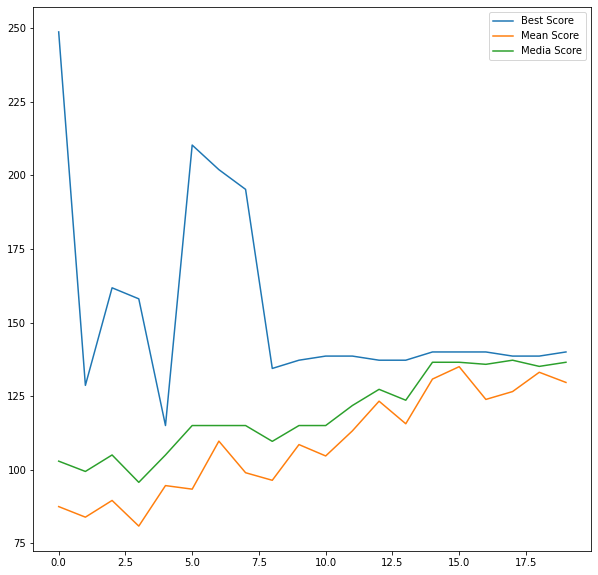
\includegraphics[scale=0.3]{images/03-cr-02-mr.png}
  \end{minipage}}
  \hfill
  \subfloat[CR = 0.2, Initial MR=0.4]{
  \begin{minipage}[c]{0.4\textwidth}
    \centering
    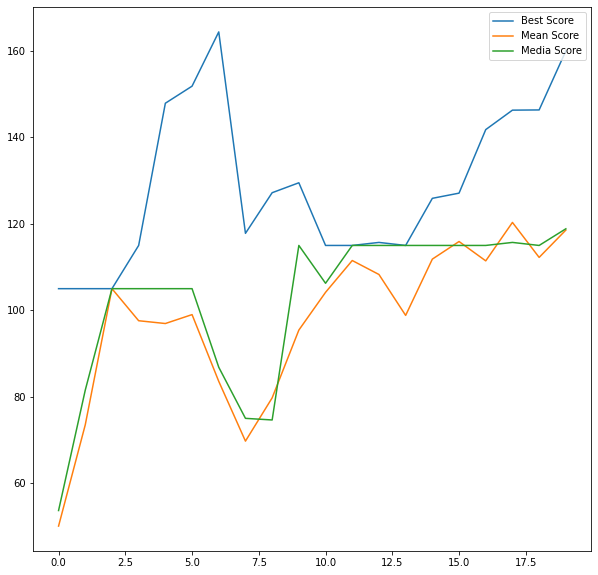
\includegraphics[scale=0.3]{images/02-cr-04-mr.png}
  \end{minipage}}
  \hfill
  \vfill
  \subfloat[CR = 0.4, Initial MR=0.3]{
  \begin{minipage}[c]{0.4\textwidth}
    \centering
    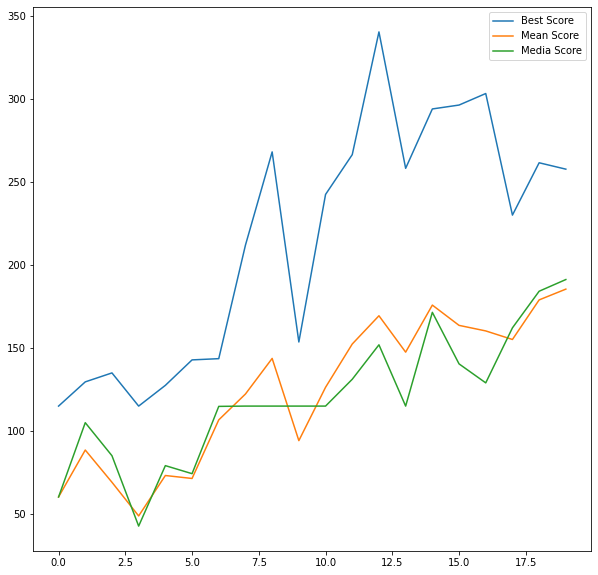
\includegraphics[scale=0.3]{images/04-cr-03-mr.png}
  \end{minipage}}
  \hfill
  \subfloat[CR = 0.4, Initial MR=0.2]{
  \begin{minipage}[c]{0.4\textwidth}
    \centering
    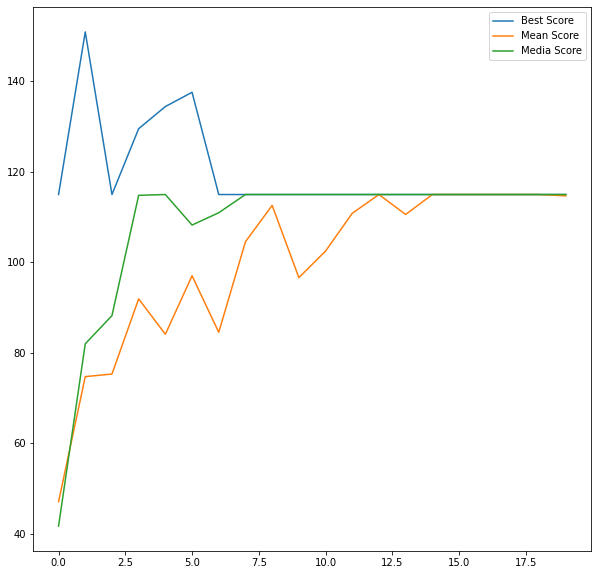
\includegraphics[scale=0.3]{images/04-cr-02-mr.png}
  \end{minipage}}
  \hfill
  \caption{CR and MR Testing (x-axis - Current Generation, y-axis - Score)}
  \label{fig:crmr}
\end{figure}

\paragraph{}


Using these determined rates both the mutation and crossover operators were tested. Initially, Option 2 from Table \ref{tab:cr} for crossover was tested. This is where an entire layer was chosen to swap with both parents, if the chance was less than the crossover rate. The results of this coincided with my initial thoughts, and the models being used are likely too small for this option to be viable. Therefore, Option 1 from Table \ref{tab:cr} was chosen, which was to randomly select an individual weight for crossover between two parents. For mutation, I tested the 3 different operators from Table \ref{tab:mr}, the resulting output graphs can be see in Fig. \ref{fig:mot}. For these results, there was 5 episodes per agent per generation, and each episode was limited to 1 life. The total number of generations was limited to 8 due to time constraints. The final mutation operator was chosen to be Option 2 (where each weight is changed by a random percentage), as this produced the most consistent results and largest scores.

\begin{figure}[ht]
  \centering
  \subfloat[Option 1]{
    \begin{minipage}[c]{0.3\textwidth}
      \centering
      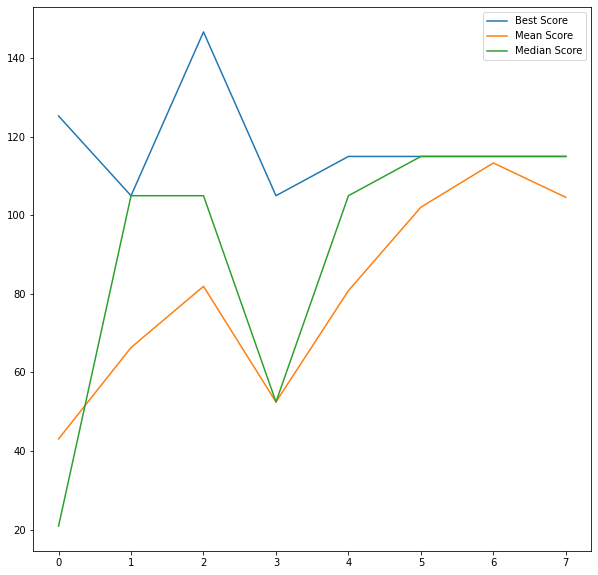
\includegraphics[scale=0.25]{images/mr-option1.png}
    \end{minipage}}
  \hfill
  \subfloat[Option 2]{
    \begin{minipage}[c]{0.3\textwidth}
      \centering
      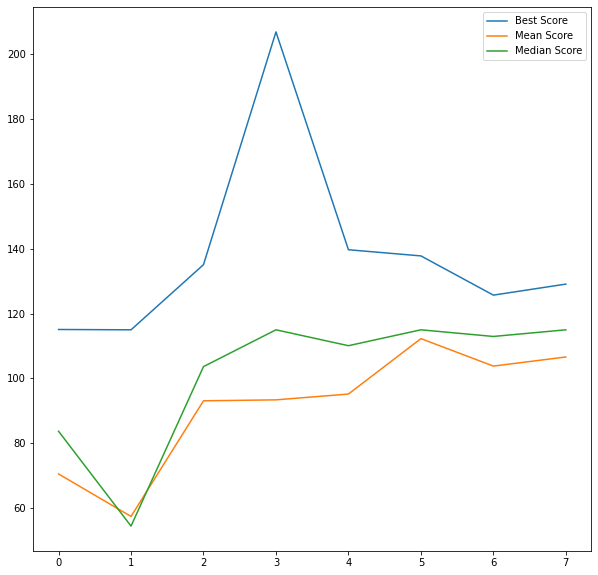
\includegraphics[scale=0.25]{images/mr-option2.png}
    \end{minipage}}
  \hfill
  \subfloat[Option 3]{
   \begin{minipage}[c]{0.3\textwidth}
     \centering
     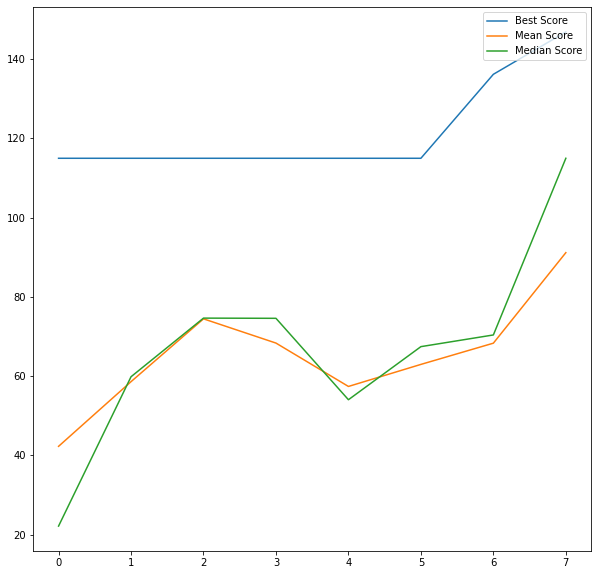
\includegraphics[scale=0.25]{images/mr-option3.png}
   \end{minipage}}
  \hfill
  \caption{Best Mutation Operator Testing - (x-axis - Current Generation, y-axis - Score)}
  \label{fig:mot}
\end{figure}


\section{Transfer Learning}

The transfer learning can be performed by initiating another instance of the Runner class with a new environment. The best agent from the final execution of the GA can be passed into this Runner to compare this agent with an agent that just takes random moves at each step. We can perfom this over N episodes, where N will be defined depending on the time constraints, and compare the results.

\paragraph{}

All code for this project can be found in this repository - https://github.com/tomcotter7/OpenAI-GeneticAlgorithms
